% =====================================================================
%  LL(1) Parser Generator — Compiler Design Presentation
%  Team 4 · 13 slides · compiles with pdflatex (Overleaf-ready)
%
%  Design: dark developer-tool aesthetic.
%  Palette: navy backgrounds, blue/cyan accents, violet highlights.
%  Built for reliability: simple TikZ, no custom math, no fragile macros.
% =====================================================================
\documentclass[aspectratio=169,11pt]{beamer}

\usepackage{xcolor}
\usepackage{tikz}
\usetikzlibrary{arrows.meta, positioning}
\usepackage{tcolorbox}
\tcbuselibrary{skins}
\usepackage{lmodern}
\usepackage[T1]{fontenc}
\usepackage{microtype}

% ----------------------- palette -----------------------
\definecolor{BgDeep}{HTML}{0B1020}
\definecolor{BgSoft}{HTML}{0F172A}
\definecolor{CardBase}{HTML}{111827}
\definecolor{CardHi}{HTML}{172033}
\definecolor{CardLine}{HTML}{1E293B}
\definecolor{PriBlue}{HTML}{2563EB}
\definecolor{CyanPop}{HTML}{06B6D4}
\definecolor{VioletPop}{HTML}{8B5CF6}
\definecolor{GreenOk}{HTML}{22C55E}
\definecolor{TextMain}{HTML}{F8FAFC}
\definecolor{TextMut}{HTML}{94A3B8}

% ----------------------- beamer chrome -----------------------
\setbeamertemplate{navigation symbols}{}
\setbeamertemplate{headline}{}
\setbeamertemplate{footline}{}
\setbeamercolor{normal text}{fg=TextMain,bg=BgDeep}
\setbeamercolor{background canvas}{bg=BgDeep}
\setbeamercolor{structure}{fg=PriBlue}
\setbeamercolor{itemize item}{fg=CyanPop}
\setbeamercolor{itemize subitem}{fg=TextMut}
\usefonttheme{professionalfonts}

\setbeamersize{text margin left=0.75cm, text margin right=0.75cm}

% ----------------------- small helpers -----------------------
% tiny uppercase label above the slide title
\newcommand{\kick}[2]{%
  {\ttfamily\fontsize{8}{9}\selectfont\bfseries\textcolor{#1}{#2}}}

% slide header: kicker + title
\newcommand{\shead}[2]{%
  \kick{CyanPop}{\uppercase{#1}}\\[1pt]
  {\fontsize{21}{25}\selectfont\bfseries\color{TextMain}#2}\\[6pt]}

% footer with page number
\newcommand{\sfoot}[1]{%
  \vfill
  \begin{tikzpicture}[remember picture,overlay]
    \draw[CardLine,line width=0.4pt]
      ([yshift=0.55cm]current page.south west) -- ([yshift=0.55cm]current page.south east);
    \node[anchor=south west,font=\ttfamily\fontsize{7}{8}\selectfont,
      text=CardLine] at ([xshift=0.75cm,yshift=0.30cm]current page.south west)
      {COMPILER DESIGN \textcolor{CardLine}{$\cdot$} TEAM 4};
    \node[anchor=south east,font=\ttfamily\fontsize{7}{8}\selectfont,
      text=CardLine] at ([xshift=-0.75cm,yshift=0.30cm]current page.south east)
      {#1\,/\,13};
  \end{tikzpicture}}

% rounded card with small mono title
\newtcolorbox{dcard}[1]{%
  enhanced, colback=CardBase, colframe=CardLine, boxrule=0.6pt,
  arc=2.5mm, left=8pt, right=8pt, top=7pt, bottom=7pt,
  title={\ttfamily\fontsize{7.5}{9}\selectfont\bfseries
         \textcolor{CyanPop}{\uppercase{#1}}},
  coltitle=CyanPop, colbacktitle=CardBase, titlerule=0pt,
  toptitle=6pt, bottomtitle=2pt}

% code/terminal panel with mono content
\newenvironment{codepanel}{%
  \begin{tcolorbox}[enhanced, colback=BgSoft, colframe=CardLine, boxrule=0.6pt,
      arc=2mm, left=10pt, right=10pt, top=8pt, bottom=8pt]}{%
  \end{tcolorbox}}

% mono text helpers
\newcommand{\mono}[1]{{\ttfamily #1}}
\newcommand{\monoC}[1]{{\ttfamily\textcolor{CyanPop}{#1}}}
\newcommand{\monoG}[1]{{\ttfamily\textcolor{GreenOk}{#1}}}
\newcommand{\monoV}[1]{{\ttfamily\textcolor{VioletPop}{#1}}}
\newcommand{\mut}[1]{{\color{TextMut}#1}}

\begin{document}

% =====================================================================
% SLIDE 1 — TITLE
% =====================================================================
\begin{frame}[plain]
  \vspace{1.1cm}
  \centering
  \kick{CyanPop}{TEAM 4 \quad$\cdot$\quad COMPILER DESIGN}\\[12pt]
  {\fontsize{30}{36}\selectfont\bfseries\color{TextMain}
   LL(1) Parser Generator}\\[10pt]
  {\fontsize{12}{17}\selectfont\mut{Design and Implementation of an LL(1)
   Parser Generator with Automatic FIRST--FOLLOW Computation,\\
   Predictive Parsing Table Construction and Syntax-Directed
   Translation}}\\[16pt]
  
\begin{tikzpicture}
    \draw[PriBlue, line width=2pt, rounded corners=1pt] (0,0) -- (2.2,0);
    \draw[CyanPop, line width=2pt, rounded corners=1pt] (2.3,0) -- (3.9,0);
    \draw[VioletPop, line width=2pt, rounded corners=1pt] (4.0,0) -- (5.2,0);
  \end{tikzpicture}\\[18pt]

  % five member placeholder cards
  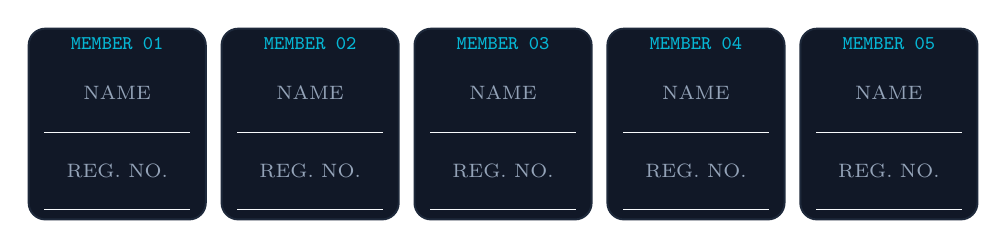
\begin{tikzpicture}
    \foreach \i in {1,...,5} {
      \node[draw=CardLine, fill=CardBase, rounded corners=6pt, line width=0.7pt,
            minimum width=2.25cm, minimum height=1.9cm, align=center]
        at ({(\i-1)*2.45}, 0) {%
          {\ttfamily\fontsize{7}{8}\selectfont\bfseries\color{CyanPop}
           MEMBER 0\i}\\[6pt]
          {\fontsize{7}{8}\selectfont\mut{NAME}}\\
          {\color{TextMain}\rule{1.85cm}{0.4pt}}\\[4pt]
          {\fontsize{7}{8}\selectfont\mut{REG. NO.}}\\
          {\color{TextMain}\rule{1.85cm}{0.4pt}}};
    }
  \end{tikzpicture}
\end{frame}

% =====================================================================
% SLIDE 2 — PROBLEM STATEMENT & OBJECTIVE
% =====================================================================
\begin{frame}
  \sfoot{2}
  \shead{The Problem}{Why build a parser generator?}
  \begin{columns}[t]
    \column{0.48\textwidth}
    \begin{dcard}{Manual construction}
      \small
      Computing FIRST and FOLLOW sets by hand is slow and error-prone.
      Every grammar change means redoing the table. Manual parsing
      tables are hard to verify and hard to reuse.\\[6pt]
      \mut{\footnotesize One slip and the whole parse breaks silently.}
    \end{dcard}
    \column{0.48\textwidth}
    \begin{dcard}{Main objective}
      \small
      Build a \textcolor{CyanPop}{generic LL(1) parser generator} in C:
      given any CFG in a documented format, it computes FIRST/FOLLOW
      automatically, builds the predictive parsing table, detects LL(1)
      conflicts, parses input strings, and performs syntax-directed
      translation.\\[6pt]
      \mut{\footnotesize Not a parser for one fixed grammar — a
      generator.}
    \end{dcard}
  \end{columns}
\end{frame}

% =====================================================================
% SLIDE 3 — SYSTEM OVERVIEW
% =====================================================================
\begin{frame}
  \sfoot{3}
  \shead{System Overview}{One pipeline, end to end}
  \vspace{0.4cm}
  \centering
  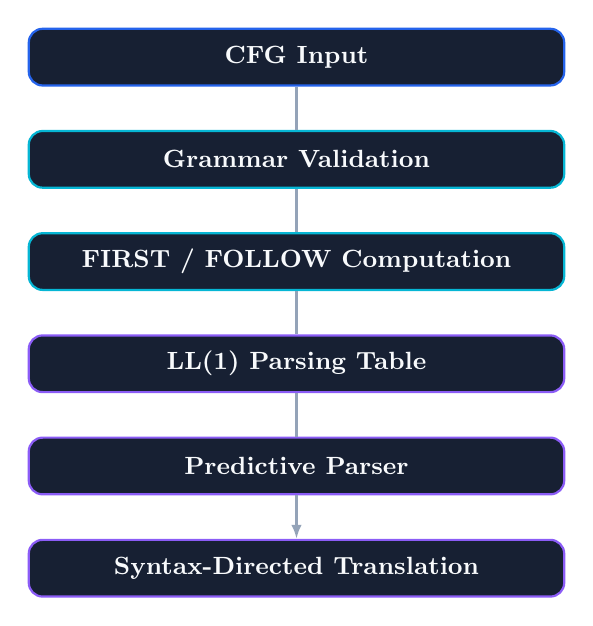
\begin{tikzpicture}[node distance=0.55cm,
      stage/.style={draw=PriBlue, fill=CardHi, rounded corners=5pt,
        line width=0.8pt, minimum width=6.8cm, minimum height=0.72cm,
        font=\small\bfseries, text=TextMain}]
    \node[stage] (a) {CFG Input};
    \node[stage, below=of a, draw=CyanPop] (b) {Grammar Validation};
    \node[stage, below=of b, draw=CyanPop] (c) {FIRST / FOLLOW Computation};
    \node[stage, below=of c, draw=VioletPop] (d) {LL(1) Parsing Table};
    \node[stage, below=of d, draw=VioletPop] (e) {Predictive Parser};
    \node[stage, below=of e, draw=VioletPop] (f) {Syntax-Directed Translation};
    \draw[-{Latex[length=5pt]}, TextMut, line width=0.8pt]
      (a) -- (b) -- (c) -- (d) -- (e) -- (f);
  \end{tikzpicture}
\end{frame}

% =====================================================================
% SLIDE 4 — PROJECT ARCHITECTURE
% =====================================================================
\begin{frame}
  \sfoot{4}
  \shead{Project Architecture}{Modular C implementation}
  \begin{columns}[t]
    \column{0.60\textwidth}
    \begin{tikzpicture}
      \foreach \i/\m in {0/{Grammar Processing}, 1/{FIRST Computation},
          2/{FOLLOW Computation}, 3/{Parsing Table},
          4/{Predictive Parser}, 5/{Syntax-Directed Translation}} {
        \pgfmathsetmacro{\x}{mod(\i,2)*5.3}
        \pgfmathsetmacro{\y}{-floor(\i/2)*1.5}
        \node[draw=CardLine, fill=CardBase, rounded corners=6pt,
              line width=0.7pt, minimum width=5.0cm, minimum height=1.15cm,
              align=center, font=\small]
          at (\x, \y)
          {\textcolor{CyanPop}{\mono{MODULE 0\the\numexpr\i+1}}}\\[2pt]
          {\color{TextMain}\m}};
    \end{tikzpicture}
    \column{0.36\textwidth}
    \begin{dcard}{Toolchain}
      \small
      \textcolor{TextMain}{Language:} \monoC{C99 / C11}\\[4pt]
      \textcolor{TextMain}{Interface:} CLI application\\[4pt]
      \textcolor{TextMain}{Structure:} modular \mono{.c}/\mono{.h} files\\[4pt]
      \textcolor{TextMain}{Build:} \monoC{gcc -Wall -Wextra}\\[4pt]
      \textcolor{TextMain}{Tests:} sample grammar suite
    \end{dcard}
  \end{columns}
\end{frame}

% =====================================================================
% SLIDE 5 — GRAMMAR PROCESSING
% =====================================================================
\begin{frame}
  \sfoot{5}
  \shead{Module 1}{Grammar processing and validation}
  \begin{columns}[t]
    \column{0.46\textwidth}
    \begin{dcard}{Sample grammar}
      \begin{codepanel}
        \mono
        E\ \ -> T Ep\\
        Ep -> + T Ep | \#\\
        T\ \ -> F Tp\\
        Tp -> * F Tp | \#\\
        F\ \ -> ( E ) | id
      \end{codepanel}
    \end{dcard}
    \column{0.50\textwidth}
    \begin{dcard}{What the module does}
      \small
      \begin{itemize}\setlength\itemsep{2pt}
        \item Reads CFG productions from file or stdin
        \item Splits alternatives on \monoC{|}
        \item Identifies non-terminals (LHS symbols), terminals, start symbol
        \item Validates: undefined symbols, missing arrows, malformed rules
      \end{itemize}
      \vspace{4pt}
      {\footnotesize\mut{\monoC{\#} = epsilon (empty string) \quad
      \monoG{\$} = input end marker}}
    \end{dcard}
  \end{columns}
\end{frame}

% =====================================================================
% SLIDE 6 — FIRST SET COMPUTATION
% =====================================================================
\begin{frame}
  \sfoot{6}
  \shead{Module 2}{FIRST set computation}
  \begin{columns}[t]
    \column{0.48\textwidth}
    \begin{dcard}{Definition and method}
      \small
      \textcolor{TextMain}{FIRST(X)} = set of terminals that can begin
      strings derived from X.\\[6pt]
      Computed by \textcolor{CyanPop}{fixed-point iteration}: repeat
      until no set changes, propagating epsilon through RHS sequences.
    \end{dcard}
    \column{0.48\textwidth}
    \begin{dcard}{Result for the sample grammar}
      \begin{codepanel}
        \mono
        FIRST(E)\ \ = \{ (, id \}\\
        FIRST(Ep) = \{ +, \# \}\\
        FIRST(T)\ \ = \{ (, id \}\\
        FIRST(Tp) = \{ *, \# \}\\
        FIRST(F)\ \ = \{ (, id \}
      \end{codepanel}
    \end{dcard}
  \end{columns}
\end{frame}

% =====================================================================
% SLIDE 7 — FOLLOW SET COMPUTATION
% =====================================================================
\begin{frame}
  \sfoot{7}
  \shead{Module 3}{FOLLOW set computation}
  \begin{columns}[t]
    \column{0.48\textwidth}
    \begin{dcard}{Definition and rules}
      \small
      \textcolor{TextMain}{FOLLOW(A)} = terminals that can appear
      immediately after A.\\[6pt]
      Three rules, iterated to a fixed point:
      \begin{itemize}\setlength\itemsep{1pt}
        \item \monoG{\$} $\in$ FOLLOW(start symbol)
        \item FIRST($\beta$)$\setminus\{\epsilon\}$
              $\subseteq$ FOLLOW(B), for $A \to \alpha B \beta$
        \item FOLLOW(A) $\subseteq$ FOLLOW(B), if $\beta$ can be empty
      \end{itemize}
    \end{dcard}
    \column{0.48\textwidth}
    \begin{dcard}{Result for the sample grammar}
      \begin{codepanel}
        \mono
        FOLLOW(E)\ \ = \{ ), \$ \}\\
        FOLLOW(Ep) = \{ ), \$ \}\\
        FOLLOW(T)\ \ = \{ +, ), \$ \}\\
        FOLLOW(Tp) = \{ +, ), \$ \}\\
        FOLLOW(F)\ \ = \{ *, +, ), \$ \}
      \end{codepanel}
    \end{dcard}
  \end{columns}
\end{frame}

% =====================================================================
% SLIDE 8 — LL(1) PARSING TABLE
% =====================================================================
\begin{frame}
  \sfoot{8}
  \shead{Module 4}{LL(1) predictive parsing table}
  \vspace{0.2cm}
  \small
  For each production $A \to \alpha$: place it in M[A, a] for every
  terminal $a$ in FIRST($\alpha$); if $\alpha$ can derive $\epsilon$,
  also place it in M[A, b] for every $b$ in FOLLOW(A).\\[8pt]
  \mut{One production per cell. A second production reaching an occupied
  cell is an \textcolor{GreenOk}{LL(1) conflict} — reported, never
  overwritten. No conflicts here: the grammar is LL(1).}

  \vspace{0.35cm}
  \centering
  {\ttfamily\footnotesize
  \renewcommand{\arraystretch}{1.45}
  \begin{tabular}{c|cccccc}
    & + & * & ( & ) & id & \$ \\ \hline
    \textcolor{PriBlue}{E}  & & & T Ep & & T Ep & \\
    \textcolor{PriBlue}{Ep} & + T Ep & & & \# & & \# \\
    \textcolor{PriBlue}{T}  & & & F Tp & & F Tp & \\
    \textcolor{PriBlue}{Tp} & \# & * F Tp & & \# & & \# \\
    \textcolor{PriBlue}{F}  & & & ( E ) & & id & \\
  \end{tabular}}
\end{frame}

% =====================================================================
% SLIDE 9 — PREDICTIVE PARSING
% =====================================================================
\begin{frame}
  \sfoot{9}
  \shead{Module 5}{Predictive parsing in action}
  \begin{columns}[t]
    \column{0.48\textwidth}
    \begin{dcard}{How the parser works}
      \small
      Stack starts with \monoG{\$ E}; input ends with \monoG{\$}.
      \begin{itemize}\setlength\itemsep{2pt}
        \item Stack top = terminal: match and pop
        \item Stack top = non-terminal: consult M[top, lookahead],
              expand RHS in reverse
        \item \monoC{\#} pops nothing; \monoG{\$} on both = accept
      \end{itemize}
    \end{dcard}
    \column{0.48\textwidth}
    \begin{dcard}{Parsing trace (excerpt)}
      \begin{codepanel}
        \footnotesize\mono
        \mut{STACK\ \ \ \ \ INPUT\ \ \ \ \ ACTION}\\
        \$ E\ \ \ \ \ \ id+id*id\$ \ \ \ E -> T Ep\\
        \$ Ep T\ \ \ \ id+id*id\$ \ \ \ T -> F Tp\\
        \$ Ep Tp id\ id+id*id\$ \ \ \ match id\\
        \monoG{\$\ \ \ \ \ \ \ \$\ \ \ \ \ \ \ \ \ \ \ accept}
      \end{codepanel}
      \vspace{2pt}
      \centering
      {\small\bfseries\color{GreenOk}INPUT ACCEPTED}
    \end{dcard}
  \end{columns}
\end{frame}

% =====================================================================
% SLIDE 10 — SYNTAX-DIRECTED TRANSLATION
% =====================================================================
\begin{frame}
  \sfoot{10}
  \shead{Module 6}{Syntax-directed translation}
  \begin{columns}[t]
    \column{0.48\textwidth}
    \begin{dcard}{Semantic actions}
      \small
      Actions fire during parsing:
      \begin{itemize}\setlength\itemsep{2pt}
        \item Terminals emit themselves to the postfix stream
        \item Operators emit after their operands
        \item Epsilon emits nothing
        \item TAC temporaries (\monoC{t1}, \monoC{t2}) are allocated as
              operators complete
      \end{itemize}
    \end{dcard}
    \column{0.48\textwidth}
    \begin{dcard}{Input: id + id * id}
      \begin{codepanel}
        \mono
        \mut{POSTFIX}\\
        id id id * +\\[6pt]
        \mut{THREE-ADDRESS CODE}\\
        t1 = id * id\\
        t2 = id + t1
      \end{codepanel}
    \end{dcard}
  \end{columns}
\end{frame}

% =====================================================================
% SLIDE 11 — IMPLEMENTATION & TECHNOLOGY
% =====================================================================
\begin{frame}
  \sfoot{11}
  \shead{Implementation}{Technology and practice}
  \begin{columns}[t]
    \column{0.48\textwidth}
    \begin{dcard}{Technology}
      \small
      \begin{itemize}\setlength\itemsep{2pt}
        \item Language: \monoC{C99 / C11}
        \item CLI application, no GUI
        \item Modular \mono{.c}/\mono{.h} per module
        \item Built with \monoC{gcc -std=c99 -Wall -Wextra -pedantic}
      \end{itemize}
    \end{dcard}
    \column{0.48\textwidth}
    \begin{dcard}{Engineering practice}
      \small
      \begin{itemize}\setlength\itemsep{2pt}
        \item Fixed-point FIRST and FOLLOW algorithms
        \item Table-driven predictive parsing
        \item Syntax-directed postfix and TAC generation
        \item Testing and debugging with multiple sample grammars,
              epsilon cases and non-LL(1) conflicts
      \end{itemize}
    \end{dcard}
  \end{columns}
\end{frame}

% =====================================================================
% SLIDE 12 — TEAM CONTRIBUTIONS
% =====================================================================
\begin{frame}
  \sfoot{12}
  \shead{Team 4}{Contributions and module ownership}
  \vspace{0.3cm}
  \centering
  {\small
  \renewcommand{\arraystretch}{1.7}
  \begin{tabular}{clll}
    \textcolor{CyanPop}{\bfseries MEMBER} &
    \textcolor{CyanPop}{\bfseries NAME} &
    \textcolor{CyanPop}{\bfseries REG. NO.} &
    \textcolor{CyanPop}{\bfseries MODULE OWNERSHIP} \\ \hline
    Member 1 & \rule{3.2cm}{0.4pt} & \rule{2.6cm}{0.4pt} & Grammar Processing / Validation \\
    Member 2 & \rule{3.2cm}{0.4pt} & \rule{2.6cm}{0.4pt} & FIRST Computation \\
    Member 3 & \rule{3.2cm}{0.4pt} & \rule{2.6cm}{0.4pt} & FOLLOW Computation \\
    Member 4 & \rule{3.2cm}{0.4pt} & \rule{2.6cm}{0.4pt} & Parsing Table / Conflict Detection \\
    Member 5 & \rule{3.2cm}{0.4pt} & \rule{2.6cm}{0.4pt} & Parser / Syntax-Directed Translation \\
  \end{tabular}}\\[10pt]
  \mut{\footnotesize Testing, integration and documentation are shared
  across the team.}
\end{frame}

% =====================================================================
% SLIDE 13 — CONCLUSION & FUTURE SCOPE
% =====================================================================
\begin{frame}
  \sfoot{13}
  \shead{Wrap-Up}{Conclusion and future scope}
  \begin{columns}[t]
    \column{0.48\textwidth}
    \begin{dcard}{Conclusion}
      \small
      \begin{itemize}\setlength\itemsep{2pt}
        \item Automated LL(1) parser generation from any CFG
        \item FIRST/FOLLOW computed to a fixed point
        \item Predictive parsing table with conflict detection
        \item Predictive parsing of input strings
        \item Syntax-directed translation: postfix and TAC
      \end{itemize}
    \end{dcard}
    \column{0.48\textwidth}
    \begin{dcard}{Future scope}
      \small
      \begin{itemize}\setlength\itemsep{2pt}
        \item Better grammar diagnostics
        \item More grammar input formats
        \item Parse-tree visualization
        \item Additional translation schemes
      \end{itemize}
      \vspace{8pt}
      \centering
      {\large\bfseries\color{TextMain} Thank You}\\[2pt]
      {\footnotesize\mut{Questions?}}
    \end{dcard}
  \end{columns}
\end{frame}

\end{document}
